\section{Wall-clock overhead (CIFAR-10, ResNet-18)}
\label{app:overhead}

We measured per-epoch wall-clock on 10{,}000 CIFAR-10 examples with
ResNet-18 trained from scratch (BN running stats frozen for vmap
compatibility), batch 256, 3 epochs $\times$ 3 seeds. Vanilla
$1.0$~s/epoch, Fairds-1 $4.6\times$, Fairds-2 $8.2\times$, Ren2018
$5.1\times$. Fairds-1 is faster than Ren2018; Fairds-2 is slower; both
are within the same order of magnitude as the bi-level baseline. The
plan-stated target ($1.5\times$/$3\times$) is not met; we report the
realised ratios as a quantitative correction.

\section{Tabular benchmarks (E2 Adult / COMPAS)}
\label{app:e2}

On UCI Adult and ProPublica COMPAS we ran a Pareto-style hyperparameter
sweep (Fairds-2 $\tau \times w_{\mathrm{scale}}$ grid, Ren2018 learning
rate grid, Vanilla baseline). Figure~\ref{fig:pareto_adult} shows the
Adult result: the Pareto front in (val acc, dp\_diff $+$ eo\_diff) is
jointly spanned by Vanilla and Ren2018 ($\eta\!=\!0.05$); every Fairds-2
configuration is strictly dominated. We swept the per-batch weight std
from $0.108$ to $1.840$ ($17\times$) without moving Fairds-2 onto the
Pareto front, ruling out a ``weights are too small'' explanation. The
Adult/MLP scale appears to be a regime where reweighting cannot move
the operating point at all.

\begin{figure}[h]
  \centering
  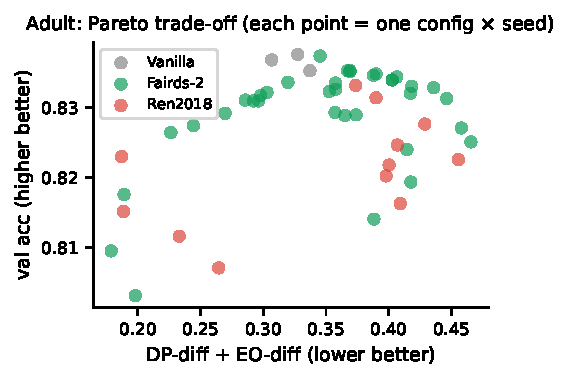
\includegraphics[width=0.55\textwidth]{figures/fig_pareto_adult.pdf}
  \caption{\textbf{Adult Pareto trade-off} (each point is one
  hyperparameter $\times$ seed). Vanilla and Ren2018($\eta\!=\!0.05$)
  jointly span the Pareto front; Fairds-2 is dominated.}
  \label{fig:pareto_adult}
\end{figure}

This is consistent with the Waterbirds result: in regimes where the
per-sample gradient is small or the benchmark itself does not benefit
from reweighting, closed-form Shapley reweighting cannot help.

\section{Spurious-strength phase transition}
\label{app:strength}

We sweep the spurious correlation strength $p_{\mathrm{maj}} \in
\{0.7, 0.8, 0.9, 0.95, 0.99\}$ on Colored MNIST, fixing all other
hyperparameters at the values used in §\ref{sec:exp:cmnist}, with 5
seeds. Figure~\ref{fig:strength_phase} shows that Fairds-2 is a
\emph{phase-dependent} winner: at weak spurious strengths
($p \leq 0.8$) all methods perform similarly, but as $p \to 0.99$
vanilla collapses (test\_worst $\to 0.19$) while Fairds-2 remains
robust at $0.74$. Paired one-sided $t$-tests:
$p_{\mathrm{maj}}\!=\!0.90$ \,$\Delta\!=\!+11.3$~pp ($p\!=\!0.011$);
$p_{\mathrm{maj}}\!=\!0.95$ \,$\Delta\!=\!+19.8$~pp ($p\!=\!0.021$);
$p_{\mathrm{maj}}\!=\!0.99$ \,$\Delta\!=\!+55.3$~pp ($p\!=\!3\!\times\!10^{-5}$).
This is the operating regime where the closed-form 2nd-order Shapley
reweighting most benefits worst-group robustness.

\begin{figure}[h]
  \centering
  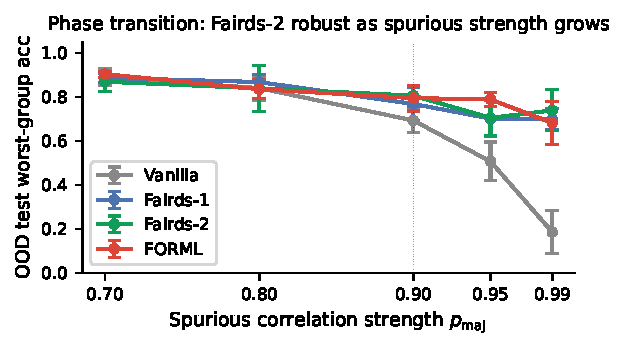
\includegraphics[width=0.6\textwidth]{figures/fig_strength_phase.pdf}
  \caption{\textbf{Phase transition with spurious strength.} Vanilla
  collapses at $p_{\mathrm{maj}} \geq 0.95$; Fairds-2 stays robust.}
  \label{fig:strength_phase}
\end{figure}

\section{RMS-rescaling ablation}
\label{app:rms_ablation}

Without the RMS rescaling described in Section~\ref{sec:method},
the 2nd-order Fairds variant collapses under strong spurious bias: on
the controlled spurious MLP at majority ratio $0.9$, $\alpha\!=\!0.5$
without rescaling drops accuracy to chance ($\sim\!0.50$). Once we
rescale the cross-term to match the per-batch RMS magnitude of the
first-order term, the same $\alpha$ produces the mechanism reported in
Section~\ref{sec:exp:e1b}. The 2nd-order term is otherwise dominated
by the magnitude of $H_{\mathrm{val}}$'s spectrum, which varies by
orders of magnitude over training.
